\section{Static cancellation, regularity and a metric primitive}\label{sec:static}

The estimates in this section concern fixed external differential scales
and varying arrow coordinates. They do not differentiate solutions of the
phase equation with respect to their initial data.

\subsection{An exact primitive in metric directions}
Fix reference inner products and determinant volume forms on $V,U,W$,
and represent positive metrics by $h_V,h_U,h_W$. The matrices in
\eqref{eq:BCLE} are computed in orthonormal frames for those metrics.
Define the entire function
\begin{equation}\label{eq:Ein}
 \Ein(b)=\int_0^1\frac{1-e^{-sb}}s\,ds,\qquad
 b\Ein'(b)=1-e^{-b}.
\end{equation}

\begin{proposition}\label{prop:primitive}
For arbitrary rectangular $D$, the function
\begin{equation}\label{eq:primitive}
 \begin{split}
 \mathcal S_{\CC}(h)
 ={}&z_0(\log\det h_V-\log\det h_U)+z_1\log\det h_W\\
 &+z_0\tr\Ein(B)-\tr(CR(B))
 \end{split}
\end{equation}
satisfies, for $\xi_q=h_q^{-1}\delta h_q$,
\begin{equation}\label{eq:primitivevariation}
 d\mathcal S_{\CC}(\xi)=
 \tr(\Omega_V\xi_V)+\tr(\Omega_U\xi_U)+\tr(\Omega_W\xi_W).
\end{equation}
\end{proposition}

\begin{proof}
Compute at orthonormal frames, where $\xi_q$ is Hermitian and the
map variations are those preceding \eqref{eq:mapflow}.
The Ein term has coefficients $-z_0(\id-P)$ on $V$ and
$z_0(\id-Q)$ on $U$. Adding the logarithmic terms gives $z_0P$
and $-z_0Q$.

The Fr\'echet derivative $\mathrm DR_B$ is self-adjoint in the trace
pairing, since $R$ is real analytic on Hermitian matrices.
Variation of $-\tr(CR(B))$ on $V$ gives
\[
 \tfrac12\{C,R(B)\}+\tfrac12\{B,\mathrm DR_B(C)\}=K_B(C).
\]
To verify the identity, diagonalize $B$. Twice the multiplier on
the left is
\[
 R(b_i)+R(b_j)+(b_i+b_j)\frac{R(b_i)-R(b_j)}{b_i-b_j}
 =2\frac{e^{-b_j}-e^{-b_i}}{b_i-b_j},
\]
with continuous values at repeated eigenvalues.
On $U$ the coefficient is
$-D\,\mathrm DR_B(C)D^\dagger=J_L(DCD^\dagger)$,
as follows by differentiating the integral defining $R$.
On $W$ it is $-\sum_j A_jR(B)A_j^\dagger$.
These are exactly \eqref{eq:coeff}.
\end{proof}

Equation~\eqref{eq:primitivevariation} specifies a primitive on the
space of metrics of each fixed object. By itself it allows an additive
constant depending on that object. Such dependence can change a
transverse moduli-space Levi form. Whenever potentials on an arrow
space are used below, their normalization is the explicit formula
\eqref{eq:primitive} at the declared reference metrics, with only the
stated acyclic subtraction. Arbitrary object-dependent functions are
not part of that normalization. Locally pluriharmonic additions do not
change the compared forms.

\subsection{Nonscalar static cancellation and first derivatives of mass}
Fix reference metrics, an orthogonal decomposition $V=H\oplus C$, and
an invertible map $F:C\to U$. Set $D=[0,F]$ and $A_j=[B_j,T_j]$.
The differential $F$ is fixed when the arrows vary. Write
\[
 P_F=F^\dagger F,\qquad L_F=FF^\dagger,\qquad
 \lambda=\sigma_{\min}(F)^2\geq\Lambda^2\geq1.
\]
The limiting cohomology coefficient $\Omega_H$ has blocks
$z_0\id+\sum_jB_j^\dagger B_j$ and
$z_1\id-\sum_jB_jB_j^\dagger$.

Use the Euclidean norm on the real and imaginary arrow entries,
whose square is the sum of squared Hilbert--Schmidt norms.
The $C^\ell$ norm uses the corresponding operator norms of real
multilinear derivatives. No derivative in $F$ or the reference metrics
is included.

\begin{proposition}\label{prop:massC1}
On every bounded arrow-coordinate ball, for fixed charges in the strict
upper half-plane and every fixed integer $\ell\geq0$,
\begin{equation}\label{eq:staticCk}
 \norm{\Omega_F-(\Omega_H\oplus0_{\ac})}_{C^\ell}
 \leq C_\ell\Lambda^{-2},\qquad
 \norm{m_F-m_H}_{C^0}\leq C_0\Lambda^{-2}.
\end{equation}
Moreover,
\begin{equation}\label{eq:massC1}
 \norm{dm_F-dm_H}_{C^0}\leq C\Lambda^{-1}.
\end{equation}
Constants may depend on the fixed dimensions, charges, ball radius and
$\ell$, but not on arrow count, the surviving stabilizer or the condition
number of $F$.
\end{proposition}

\begin{proof}
The nonscalar blocks are given by \eqref{eq:adaptedcoeff}, with
$H_j=B_j$. Spectral calculus gives
\[
 \norm{R(P_F)}\leq\lambda^{-1},\qquad
 \norm{e^{-P_F}}=\norm{e^{-L_F}}\leq e^{-\lambda},\qquad
 \norm{K_{P_F}(C)}_{\HS}\leq e^{-\lambda}\norm C_{\HS}.
\]
For the degree-one term take a singular-value decomposition of $F$,
with squared singular values $b_i\geq\lambda$. The multiplier on
$C_{ij}$ in $J_{L_F}(FCF^\dagger)$ is
\[
 \sqrt{b_ib_j}\int_{\substack{s,t\geq0\\s+t\leq1}}
 e^{-sb_i-tb_j}\,ds\,dt
 \leq\frac1{\sqrt{b_ib_j}}\leq\lambda^{-1}.
\]
This bounds its Hilbert--Schmidt operator norm independently of the
largest singular value. All arrow expressions are quadratic.
Tuple Cauchy--Schwarz bounds their first two derivatives independently
of the number of arrows, and higher derivatives vanish. Norm conversion
in the fixed output dimensions proves the coefficient bound in
\eqref{eq:staticCk}, first with $\lambda^{-1}$ in place of $\Lambda^{-2}$.
The trace-norm triangle inequality gives the mass bound.

Every block is invertible at finite $F$: its signed imaginary part is
a positive scalar times $\id$, $e^{-P_F}$ or $e^{-L_F}$.
The trace norm $N(Z)=\norm Z_1$ is smooth on invertible matrices and
convex \cite{lewis95}. Its first derivative satisfies
$|DN_Z(H)|\leq\norm H_1$, while $D^2N_Z(H,H)\geq0$.
Along any real unit arrow direction,
\[
 \frac{d^2}{dt^2}N(\Omega(y+tv))\geq-\norm{\Omega''(y+tv)}_1.
\]
The second derivatives of the coefficients are uniformly bounded on a
ball of radius $R+1$. The cohomology mass has a bounded Hessian there,
because its blocks have uniformly positive imaginary parts.
Thus $f_F=m_F-m_H$ satisfies $D^2f_F\geq-L_R\id$, uniformly in $F$.
For $|y|\leq R$, $|v|=1$ and $0<h\leq1$, integration gives
\[
 df_F(y)v\leq\frac{f_F(y+hv)-f_F(y)}h+\frac{L_Rh}{2}
 \leq\frac{2C_0}{h\lambda}+\frac{L_Rh}{2}.
\]
Take $h=\lambda^{-1/2}$ and replace $v$ by $-v$ for the other sign.
This proves \eqref{eq:massC1}. No uniform upper Hessian bound near a
singular acyclic coefficient has been used.
\end{proof}

The map-dependent part of the primitive is exactly
\begin{equation}\label{eq:staticprimitive}
 z_0\tr\Ein(P_F)-\sum_j\norm{B_j}_{\HS}^2
 -\sum_j\tr\bigl(T_jR(P_F)T_j^\dagger\bigr).
\end{equation}
The first term is independent of the arrows at fixed $F$.
After its declared subtraction, the primitive has the same
$C^\ell$ error $O_\ell(\Lambda^{-2})$ for every fixed $\ell$.
Section~\ref{sec:geometry} states the relative normalization including
the metric determinant terms. This subtraction is not constant along
a full metric orbit where the norm of $D$ changes.
At phase $\pi/2$ and the charges $-1+\ii$, $1+\ii$, the map-dependent
real function at fixed $F$ is
$\sum_j\norm{B_j}_{\HS}^2+\sum_j\tr(T_jR(P_F)T_j^\dagger)$,
a positive Hermitian quadratic form in the arrows. Positivity when the
differential varies is a separate question, addressed below.

\subsection{A shrinking-scale profile and failure of higher derivatives}
For the rest of this subsection let $H=W=C=U=\CC^2$,
$D=[0,\Lambda\id]$, $z_0=-1+\ii$ and $z_1=1+\ii$. Put
\[
 p=e^{-\Lambda^2},\qquad
 \rho_\Lambda=R(\Lambda^2)=\frac{1-p}{\Lambda^2}.
\]
Return to the balanced family \eqref{eq:balancedfamily} and choose the constant nonzero mixing
\begin{equation}\label{eq:profilemixing}
 T_1=\id,\qquad T_2=-\sigma_z,\qquad T_3=\id .
\end{equation}
All three are invertible and $\sum_j\norm{T_j}_{\HS}^2=6$.
Here $\sum_jT_j^\dagger T_j=\sum_jT_jT_j^\dagger=3\id$,
$\sum_jB_j^\dagger T_j=c\epsilon\sigma_x$ and $m_H=4$.
The source coefficient is a direct sum, after a constant unitary
change and permutation, of two unitarily conjugate matrices
\[
 Z_\pm=\begin{pmatrix}\ii&\pm u\\\pm u&p(2+\ii)\end{pmatrix},
 \qquad u=\rho_\Lambda c\epsilon .
\]
Since $\det Z_\pm=-p-u^2+2\ii p$ and
$\tr(Z_\pm^\dagger Z_\pm)=1+5p^2+2u^2$,
\begin{equation}\label{eq:exactmassprofile}
 \begin{split}
 g_p(y)&=\sqrt{1+5p^2+2y+2\sqrt{5p^2+2py+y^2}},\\
 m_\Lambda(\epsilon)
 &=2g_p\left(\frac{\rho_\Lambda^2\epsilon^2}{2+\epsilon^2}\right)
   +2\sqrt{(3\rho_\Lambda-2p)^2+p^2}+2\sqrt{1+9\rho_\Lambda^2}.
 \end{split}
\end{equation}
All $\epsilon$ derivatives occur in the first summand.

\begin{proposition}\label{prop:profile}
Let $s_\Lambda=\sqrt{2p}/\rho_\Lambda$. For each compact real interval $I$
and each fixed nonnegative integer $k$,
\begin{equation}\label{eq:profilelimit}
 \frac{m_\Lambda(s_\Lambda\xi)-m_\Lambda(0)}{2p}
 \longrightarrow
 P(\xi):=\xi^2+\sqrt{(1+\xi^2)^2+4}-\sqrt5
 \quad\text{in }C^k(I).
\end{equation}
In particular,
\begin{align}
 \partial_\epsilon^3(m_\Lambda-m_H)(s_\Lambda)
 &\sim\frac34\,\frac{e^{\Lambda^2/2}}{\Lambda^6},\label{eq:C3failure}\\
 \partial_\epsilon^4(m_\Lambda-m_H)(0)
 &\sim\frac{24}{5\sqrt5}\,
              \frac{e^{\Lambda^2}}{\Lambda^8}.\label{eq:C4failure}
\end{align}
Thus uniform $C^3$ convergence fails on every fixed interval
$[0,\epsilon_0]$ with $\epsilon_0>0$.
\end{proposition}

\begin{proof}
Put $\eta_\Lambda=p/\rho_\Lambda^2$,
$w_\Lambda(\xi)=\xi^2/(1+\eta_\Lambda\xi^2)$ and
$H(w)=w+\sqrt{5+2w+w^2}$.
At $\epsilon=s_\Lambda\xi$ the argument of $g_p$ is $pw_\Lambda$.
Rationalizing the outer square root in \eqref{eq:exactmassprofile}
gives the exact expression
\begin{equation}\label{eq:rationalprofile}
 P_\Lambda(\xi):=\frac{m_\Lambda(s_\Lambda\xi)-m_\Lambda(0)}{2p}
 =\frac{2H(w_\Lambda(\xi))+5p}
        {\sqrt{1+2pH(w_\Lambda(\xi))+5p^2}+1}-\sqrt5.
\end{equation}
Since $p\to0$ and $\eta_\Lambda\to0$, the right side is a smooth
function of $(p,\eta_\Lambda,\xi)$ near $(0,0,I)$.
Its square-root arguments stay bounded away from zero.
This proves \eqref{eq:profilelimit}; in fact
$\norm{P_\Lambda-P}_{C^k(I)}
\leq C_{I,k}(p+\eta_\Lambda)=O_{I,k}(\Lambda^4e^{-\Lambda^2})$.

The exact derivative relation is
\[
 \partial_\epsilon^k m_\Lambda(s_\Lambda\xi)
 =2p\,s_\Lambda^{-k}P_\Lambda^{(k)}(\xi),\qquad k\geq1.
\]
Direct differentiation gives $P'''(1)=3\sqrt2/4$.
For example, for $Q(\xi)=\xi^4+2\xi^2+5$, its value and first three
derivatives at $1$ are $8,8,16,24$; substituting them in the third
derivative of $\sqrt Q$ gives the stated value.
Therefore the third derivative is asymptotic to
$3\rho_\Lambda^3/(4\sqrt p)$ at $\epsilon=s_\Lambda$, which proves
\eqref{eq:C3failure}. This point tends to zero through positive values.

For the derivative at zero set $d=1+\sqrt5p$ and $A_0=1+1/\sqrt5$.
At fixed $p>0$, expansion of the exact formula gives
\[
 g_p(y)=d+\frac{A_0}{d}y+
 \left(\frac{2}{5\sqrt5pd}-\frac{A_0^2}{2d^3}\right)y^2+O_p(y^3).
\]
Since $y=\rho_\Lambda^2\epsilon^2/(2+\epsilon^2)$, it follows exactly that
\[
 \partial_\epsilon^4m_\Lambda(0)
 =12\left[-\frac{A_0}{d}\rho_\Lambda^2+
 \left(\frac{2}{5\sqrt5pd}-\frac{A_0^2}{2d^3}\right)\rho_\Lambda^4\right].
\]
Using $\rho_\Lambda\sim\Lambda^{-2}$ and $p=e^{-\Lambda^2}$ proves
\eqref{eq:C4failure}.
\end{proof}

\begin{corollary}\label{cor:sharpregularity}
For the family \eqref{eq:profilemixing}, $m_\Lambda\to4$ in $C^2(I)$
on every compact real interval $I$. More precisely,
\[
 \norm{m_\Lambda-4}_{C^2(I)}=O_I(\Lambda^{-2}),\qquad
 \norm{m_\Lambda'}_{C^0(I)}+\norm{m_\Lambda''}_{C^0(I)}
 =O_I(\Lambda^{-4}).
\]
For every $\epsilon_0>0$ and $0<\alpha\leq1$, however,
the H\"older seminorm
$[m_\Lambda'']_{C^{0,\alpha}([0,\epsilon_0])}$ tends to infinity.
\end{corollary}

\begin{proof}
Put $f(\epsilon)=\epsilon^2/(2+\epsilon^2)$,
$y=\rho_\Lambda^2f(\epsilon)$ and
$h(y)=\sqrt{(y+p)^2+4p^2}$. For $y\geq0$ set
$A(y)=1+(y+p)/h(y)$. Then $g_p\geq1$, $1\leq A\leq2$ and
\[
 g_p'=A/g_p,\qquad
 g_p''=\frac{4p^2}{g_ph^3}-\frac{A^2}{g_p^3}.
\]
Moreover,
\[
 (f')^2=\frac{16f}{(2+\epsilon^2)^3}\leq2f,\qquad
 \frac{p^2y}{h^3}\leq\frac{p^2y}{(p+y)^3}\leq1.
\]
Only $2g_p(y)$ varies with $\epsilon$ in
\eqref{eq:exactmassprofile}. Therefore
\[
 |m_\Lambda'|\leq4\rho_\Lambda^2|f'|,\qquad
 |m_\Lambda''|\leq
 2\rho_\Lambda^4(f')^2\left(\frac{4p^2}{h^3}+4\right)
 +4\rho_\Lambda^2|f''|\leq C_I\rho_\Lambda^2.
\]
These are direct estimates on the fixed interval $I$.
Together with \eqref{eq:staticCk}, they prove the $C^2$ assertions.

For the H\"older claim, the exact rescaling gives
$m_\Lambda''(s_\Lambda\xi)=\rho_\Lambda^2P_\Lambda''(\xi)$.
Direct differentiation of $P$ gives
\[
 P''(0)=2+\frac2{\sqrt5},\qquad
 P''(1)=2+\frac3{\sqrt2},\qquad
 \Delta:=\frac3{\sqrt2}-\frac2{\sqrt5}>0.
\]
Since $s_\Lambda\to0$, both $0$ and $s_\Lambda$ lie in
$[0,\epsilon_0]$ for all large $\Lambda$. Hence
\begin{equation}\label{eq:holderfailure}
 [m_\Lambda'']_{C^{0,\alpha}([0,\epsilon_0])}
 \geq\frac{|m_\Lambda''(s_\Lambda)-m_\Lambda''(0)|}{s_\Lambda^\alpha}
 \sim2^{-\alpha/2}\Delta\,
 \frac{e^{\alpha\Lambda^2/2}}{\Lambda^{4+2\alpha}}\longrightarrow\infty.
\end{equation}
The asymptotic equivalence concerns the displayed two-point quotient.
\end{proof}

This is a derivative obstruction in the actual parameter of
\eqref{eq:balancedfamily}, with fixed reference metrics and fixed mixing.
The family extends smoothly to negative $\epsilon$, so derivatives at
zero are unambiguous. It is not asserted that $\epsilon$ is a smooth
coordinate on a coarse moduli quotient. The analytic singular scale
comes from the acyclic coefficient approaching zero; a changing
stabilizer alone is not an explanation of trace-norm singularities.
The fixed-interval $C^2$ bound is specific to this family. It does not
settle a general uniform $C^2$ estimate on the full arrow-coordinate ball.

\begin{figure}[ht]
\centering
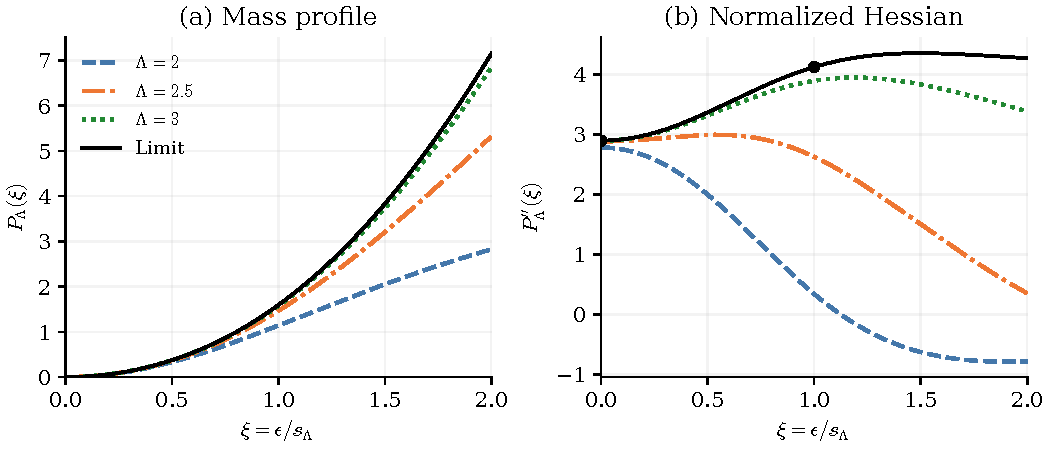
\includegraphics[width=\textwidth]{figures/output/mass-profile.pdf}
\caption{The exact normalized mass difference $P_\Lambda$ and normalized
Hessian $P_\Lambda''$, with their limits $P$ and $P''$.
The marked limiting Hessian values at $\xi=0,1$ differ by $\Delta$;
their original parameter separation tends to zero. The coordinate scale is
$s_\Lambda=\sqrt{2p}/\rho_\Lambda\sim\sqrt2\Lambda^2e^{-\Lambda^2/2}$.
The curves illustrate a proved static limit; they are not numerical
phase-flow trajectories.}\label{fig:profile}
\end{figure}
\FloatBarrier

\subsection{A negative ambient Levi direction}\label{subsec:levi}
For a phase angle $\theta\in(0,\pi)$, the real phase combination in
\cite[\S5.1]{hkkp26} is
$-\Rea\mathcal S_{\CC}+\cot\theta\,\Ima\mathcal S_{\CC}$.
On a complex gauge orbit the logarithmic determinant terms are locally
pluriharmonic. Its map-dependent candidate potential is therefore
\begin{equation}\label{eq:realpotential}
 \mathcal K_\theta(A,D)=\tr(CR(B))+c_\theta\tr\Ein(B),\qquad
 c_\theta=-\Rea z_0+\cot\theta\,\Ima z_0 .
\end{equation}
This formula is a construction from the explicit primitive; it is not
an assertion that \cite[\S5.4]{hkkp26} proves its ambient positivity.

\begin{proposition}\label{prop:negativelevi}
For $z_0=-1+\ii$, $z_1=1+\ii$ and $\theta=\pi/2$, the potential
\eqref{eq:realpotential} has a negative Levi direction on a complex
gauge orbit of the mixed family, for every $\Lambda>0$ and every
$\epsilon\in[0,1]$.
\end{proposition}

\begin{proof}
On one scalar acyclic summand put $a=|A|^2$, $b=|D|^2$.
The restriction of the potential is $aR(b)+c\Ein(b)$.
Its $A\overline A$ Levi entry is $R(b)>0$.
The Schur complement of that entry is
\begin{equation}\label{eq:levischur}
 e^{-b}[c-a\rho(b)],\qquad
 \rho(b)=\frac{b-1+e^{-b}}{b(1-e^{-b})}.
\end{equation}
Indeed the $D\overline D$ entry is
$a(R'+bR'')+ce^{-b}$, and the squared mixed entry divided by
$R$ is $ab(R')^2/R$; using $bR'=e^{-b}-R$ gives
\eqref{eq:levischur}.
For $b>0$, $\rho(b)>1/2$: the sign of $2\rho-1$ is the sign
of $b-2+(b+2)e^{-b}$, whose derivative is
$1-(b+1)e^{-b}>0$ and whose value at zero is zero.
Thus $c=1$, $a=4$ gives a negative direction for every $b>0$.

Realize this scalar restriction by taking $T_1=2\id$ and $T_2=T_3=0$
while keeping the balanced $B_j$ fixed. Vary one acyclic diagonal
entry of $D$ and the corresponding entry of $T_1$.
Independent nonzero complex rescalings of that acyclic source line
and its degree-one target line realize these two local variables
within one complex gauge orbit. Their potential is the scalar
expression above plus a constant, proving the assertion.
\end{proof}

An object-dependent additive constant cannot repair this negative
direction along the same metric orbit. The proposition obstructs a
generally plurisubharmonic ambient potential with the prescribed
phase primitive. It does not exclude a positive limiting cohomology
metric or every possible construction made directly on a quotient.

\subsection{Quantities and derivative domains}
For clarity, the static estimates concern the following distinct
objects, at fixed external $D=[0,F]$, $\sigma_{\min}(F)\geq\Lambda$,
and fixed reference metrics. The profile rows further specialize to
$F=\Lambda\id$ and the indicated family:

\begin{center}
\begin{adjustbox}{max width=\textwidth,center}
\begin{tabular}{lll}
\toprule
Quantity & Coordinate derivatives & Conclusion\\
\midrule
Coefficient $\Omega_F$ & bounded real $B,T$ coordinates
 & $C^k$ error $O_k(\Lambda^{-2})$\\
Relative primitive & the same coordinates
 & $C^k$ error $O_k(\Lambda^{-2})$\\
Trace-norm mass & the same coordinates
 & $C^0$ error $O(\Lambda^{-2})$, $C^1$ error $O(\Lambda^{-1})$\\
Mass in \eqref{eq:profilemixing} & surviving parameter $\epsilon$
 & $C^2$ convergence; $C^{2,\alpha}$ seminorms diverge\\
Normalized profile & $\xi=\epsilon/s_\Lambda$ on compact intervals
 & $C^k$ convergence for every fixed $k$\\
\bottomrule
\end{tabular}
\end{adjustbox}
\end{center}
No all-orders derivative conclusion for
$(\Omega_\Lambda\Omega_\Lambda^\dagger)^{1/2}$, the polar phase,
or an actual flow trajectory is contained in this table.
